\documentclass[conference]{IEEEtran}
\IEEEoverridecommandlockouts
% The preceding line is only needed to identify funding in the first footnote. If that is unneeded, please comment it out.
\usepackage{cite}
\usepackage{amsmath,amssymb,amsfonts}
\usepackage{algorithmic}
\usepackage{graphicx}
\usepackage{textcomp}
\usepackage{xcolor}
\usepackage{float}
\def\BibTeX{{\rm B\kern-.05em{\sc i\kern-.025em b}\kern-.08em
    T\kern-.1667em\lower.7ex\hbox{E}\kern-.125emX}}
\begin{document}

\title{Sensors Lab Conference}

\author{\IEEEauthorblockN{1\textsuperscript{st} Gabriele Paris}
\IEEEauthorblockA{\textit{Physic department} \\
\textit{Universiteit Antwerpen}\\
Antwerp, Belgium \\
gabriele.paris@student.uantwerpen.be}
\and
\IEEEauthorblockN{2\textsuperscript{nd} Given Name Surname}
\IEEEauthorblockA{\textit{dept. name of organization (of Aff.)} \\
\textit{name of organization (of Aff.)}\\
City, Country \\
email address or ORCID}
\and
\IEEEauthorblockN{3\textsuperscript{rd} Given Name Surname}
\IEEEauthorblockA{\textit{dept. name of organization (of Aff.)} \\
\textit{name of organization (of Aff.)}\\
City, Country \\
email address or ORCID}
}

\maketitle

\begin{abstract}
To write
\end{abstract}

\begin{IEEEkeywords}
6TiSCH, Contiki-NG, Energest, Zolertia
\end{IEEEkeywords}

\section{Introduction}
To write

\section{Analysing the 6TiSCH energy consumption}
\label{section:task1}
In the first analysis, we compared the energy consumption during a certain time period of the entire 6TiSCH stack to when only enabling the TSCH MAC layer (without link-layer security) after network convergence.\\
For both analyses, we report on the consumption of the root and the leaf node separately.\\
Following we remark differences in energy consumption between the root and the leaf node.

\subsection{Only TSCH MAC layer}
The basic setup for the following analysis is a root (coordinator) node that sends packets to a leaf node at a rate of 1 packet of 4 bytes per second.\\
Note that the root node has no event routine related to data reception. In the same way, the leaf node has no code which permits data transmission.\\
Both nodes are configured to measure the energy consumption by the Energest\footnote{https://github.com/contiki-ng/contiki-ng/wiki/Documentation:-Energest} module available in Contiki-ng\footnote{https://github.com/contiki-ng}.
The energy consumption is measured referring to the following formula:
\begin{equation}
	E_{tot}=\sum_{c \in comp}^{N_{c}}E_{c}=\sum_{c \in comp}^{N_{c}}I_c  \cdot V_{cc} \cdot t
\end{equation}
Where $V_{cc}$ is the supply voltage, fixed as a constant at the value $3.3V$.\\
And the single current consumption is obtained from the table \ref{tab:CurrentConsumption}\cite{inproceedings}.\\
\begin{table}[htbp]
	\begin{center}
		\begin{tabular}{ccc}
			\hline
			\textbf{State}    & \textbf{\begin{tabular}[c]{@{}c@{}}CC2538\\ datasheet\end{tabular}} & \textbf{\begin{tabular}[c]{@{}c@{}}Device\\ profiling\end{tabular}} \\ \hline
			\textbf{CPU}      & 20 mA                                                               & 15.35mA                                                             \\
			\textbf{LPM}      & 0.6 mA                                                              & 9.59 mA                                                             \\
			\textbf{Deep LPM} & 0.0013 mA                                                           & 2.58 mA                                                             \\
			\textbf{LISTEN}   & 24 mA                                                               & 28.32 mA                                                            \\
			\textbf{Rx}       & 27 mA                                                               & 30.14 mA                                                            \\
			\textbf{Tx}       & 34 mA                                                               & 31.12 mA                                                            \\ \hline
		\end{tabular}
	\end{center}
	\caption{Current draw for the TX and RX states using the CSMA
		protocol and the current drawn for TX and RX time slots using TSCH as MAC
		protocol, both when using the CC2538 radio.\cite{inproceedings}}
	\label{tab:CurrentConsumption}
\end{table}
To perform the first test only the TSCH MAC layer is enabled the rest of the stack is unused, including the security link-layer.\\
Physically speaking in this first test there is no need to measure the energy consumption variation given the distance, therefore the physical setup of the experiment consists of two Zolertia  Remote RevB boards placed at a fixed distance of approximately 10 cm.\\
At first, we have measured the energy consumption relative to the leaf node, which is only listening for data.
In figure \ref{fig:RXConsumptionTime} is possible to see the energy consumption during a period of around 27 minutes.
\begin{figure}[]
	\centering
	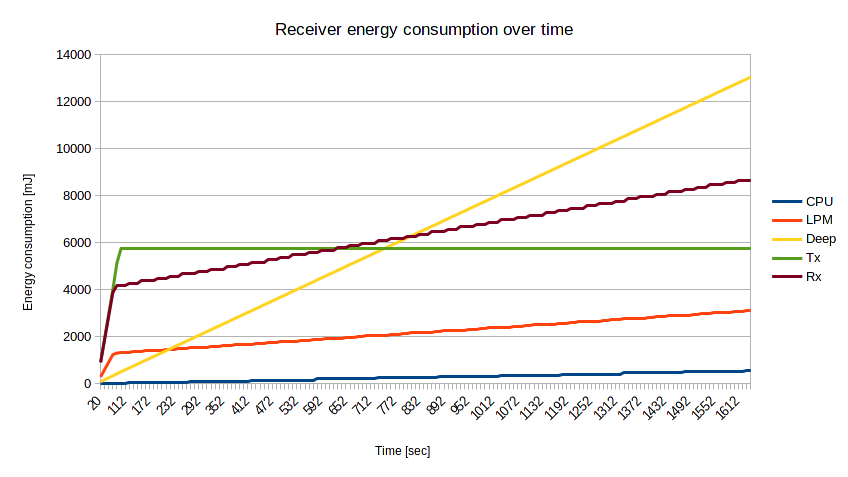
\includegraphics[width=.5\textwidth,keepaspectratio]{RXConsumptionTime.png}
	\caption{Zolertia leaf node energy consumption over time.}
	\label{fig:RXConsumptionTime}
\end{figure}
What is possible to notice is that most of the energy is used in deep sleep mode.\\
Then leaf node in this configuration requires only to listen, is therefore understandable that the majority of the time is spent in the lowest energy configuration, hence is important to notice that as referenced in table \ref{tab:CurrentConsumption} the deep state mode is the less energy consuming component, the board is prone to switch in this state as soon as possible to save battery.\\
In figure \ref{fig:RXConsumptionComponent} is shown the average energy consumption per component.\\
\begin{figure}[]
	\centering
	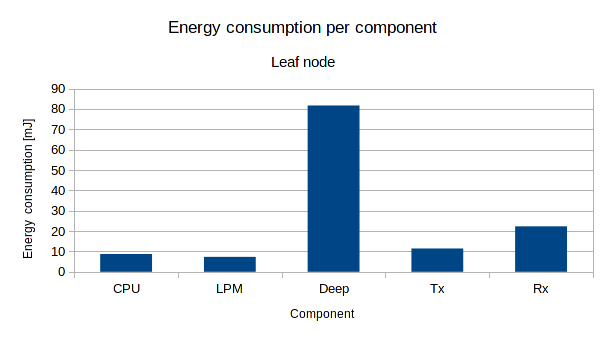
\includegraphics[width=.5\textwidth,keepaspectratio]{RXConsumptionComponent.png}
	\caption{Zolertia leaf node average energy consumption per component.}
	\label{fig:RXConsumptionComponent}
\end{figure}
Then we have performed the same experiment regarding the root coordinator node, in the same configuration for the leaf node we have measured the energy consumption over time \ref{fig:TXConsumptionTime} and per component \ref{fig:TXConsumptionComponent}.
\begin{figure}[H]
	\centering
	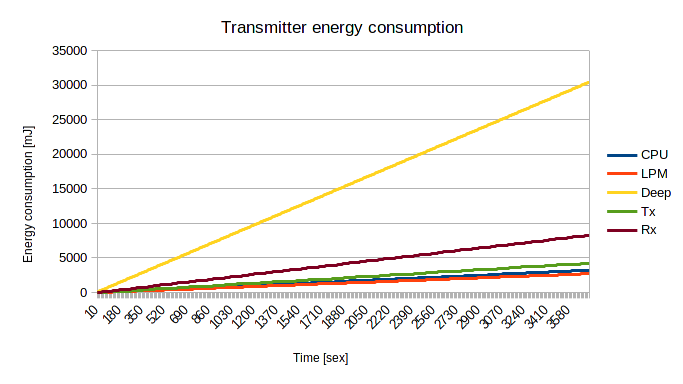
\includegraphics[width=.5\textwidth,keepaspectratio]{TXConsumptionTime.png}
	\caption{Zolertia root node energy consumption over time.}
	\label{fig:TXConsumptionTime}
\end{figure}
The first thing that is possible to notice is that the energy consumption of the transmitter continues to rise, due to the program on the root node itself, that as explained in the section \ref{section:task1} is required to send data to the leaf node.\\
As before analyzing the breakdown of the energy consumption shows us that the state of deep sleep is the favorite for the component.
\begin{figure}[]
	\centering
	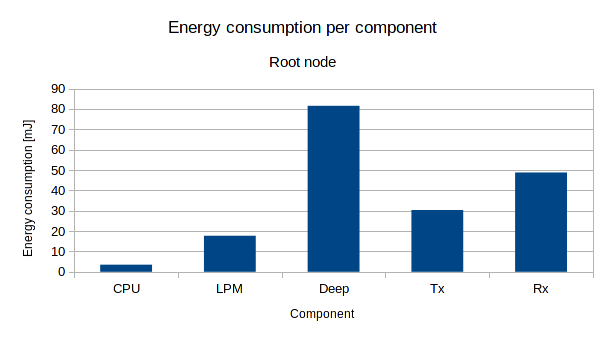
\includegraphics[width=.5\textwidth,keepaspectratio]{TXConsumptionComponent.png}
	\caption{Zolertia root node average energy consumption per component.}
	\label{fig:TXConsumptionComponent}
\end{figure}
What is interesting to notice is the conspicuous increase of energy consumption in the root node in comparison to the leaf node, in the table \ref{tab:nodeEnergyComparison1} have been reported a comparison between the two nodes average energy consumption per component.
\begin{table}[H]
	\begin{center}
		\begin{tabular}{cccccc}
			\hline
			\textbf{Board} & \textbf{CPU} & \textbf{LPM} & \textbf{Deep} & \textbf{Tx} & \textbf{Rx} \\ \hline
			\textbf{Leaf}  & 8,738 mJ        & 7,337 mJ       & 81,697 mJ       & 11,430 mJ     & 22,326 mJ     \\
			\textbf{Root}  & 3,503 mJ       & 17,716 mJ      & 81,553 mJ       & 30,352 mJ     & 48,792 mJ     \\ \hline
		\end{tabular}
	\end{center}
	\caption{Energy consumption per component per node on average.}
	\label{tab:nodeEnergyComparison1}
\end{table}
As the last measurement, the boards have been programmed to run the same code, this receives and sends messages with an interval of around 8 seconds.\\
The boards have been running for a half an hour, the total consumption has been recorded and shown in table \ref{tab:RXTXConsumptionComponent}.\\
\begin{table}[H]
	\begin{center}
		\begin{tabular}{cccccc}
			\hline
			\textbf{Board}         & \textbf{CPU} & \textbf{LPM} & \textbf{Deep} & \textbf{Tx} & \textbf{Rx} \\ \hline
			\textbf{Leaf} & 2127 mJ      & 68768 mJ     & 18858 mJ      & 227471 mJ   & 220308 mJ   \\
			\textbf{Root} & 2127 mJ      & 68009 mJ     & 18662 mJ      & 225109 mJ   & 217921 mj   \\ \hline
		\end{tabular}
	\end{center}
	\caption{Root and leaf node running the same program, power comparison per component.}
	\label{tab:RXTXConsumptionComponent}
\end{table}
\subsection{Full stack}
The next experiment is as cited in the section \ref{section:task1} introduction related to the energy consumption once the full 6TiSCH stack has been enabled (except for the security layer).\\
The setup of this experiment is similar to the previous one.
Two boards 10cm apart from each other are running the same source code.\\
In this scenario, we have a coordinator node and a leaf node. No messages are exchanged between the two if not for standard 6TiSCH service messages.\\
As before is reported the time cumulative energy consumption regarding leaf and root node. 
\begin{figure}[H]
	\centering
	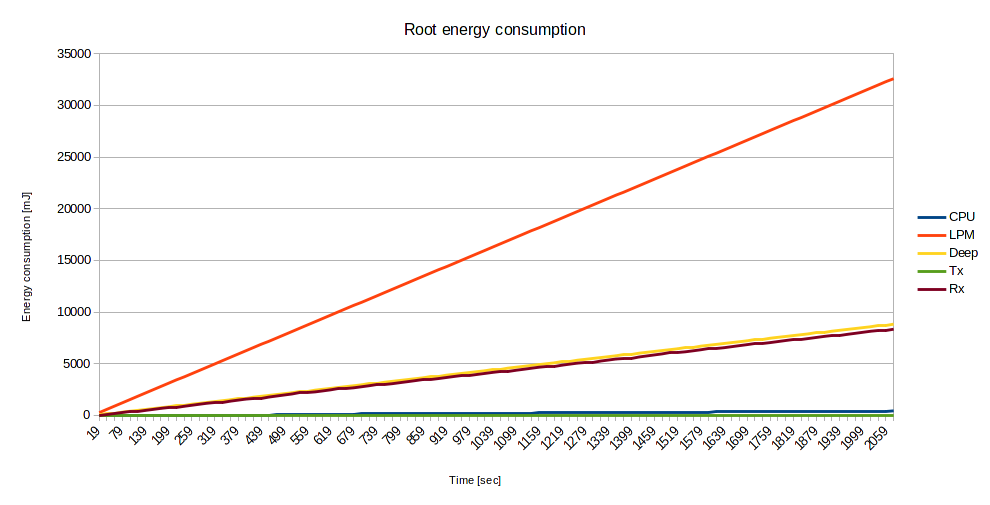
\includegraphics[width=.5\textwidth,keepaspectratio]{RootConsumptionTime.png}
	\caption{Zolertia root node energy consumption over timem full 6TiSCH stack.}
	\label{fig:RootConsumptionTime}
\end{figure}
\begin{figure}[H]
	\centering
	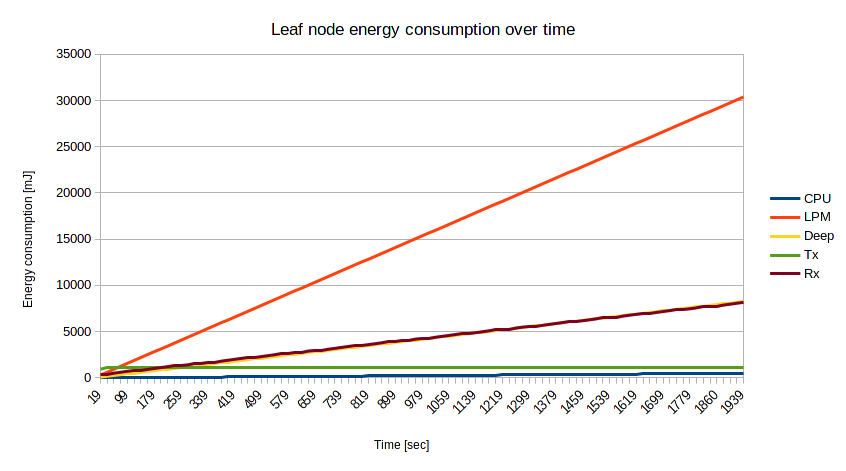
\includegraphics[width=.5\textwidth,keepaspectratio]{LeafConsumptionTime.png}
	\caption{Zolertia leaf node energy consumption over timem full 6TiSCH stack.}
	\label{fig:RootConsumptionTime}
\end{figure}
After a time analysis we provide a breakdown of the single components energy consumption.
\begin{figure}[htbp]
	\centering
	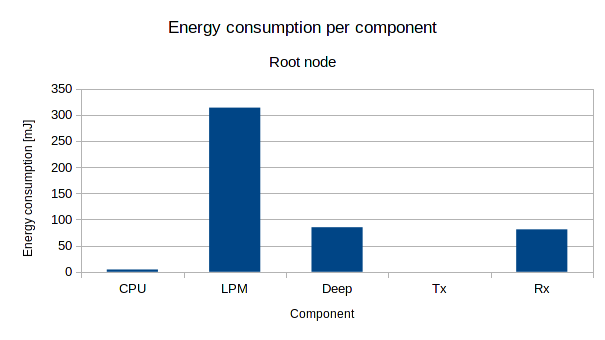
\includegraphics[width=.5\textwidth,keepaspectratio]{RootConsumptionComponent.png}
	\caption{Zolertia root node average energy consumption per component.}
	\label{fig:RootConsumptionComponent}
\end{figure}
\begin{figure}[htbp]
	\centering
	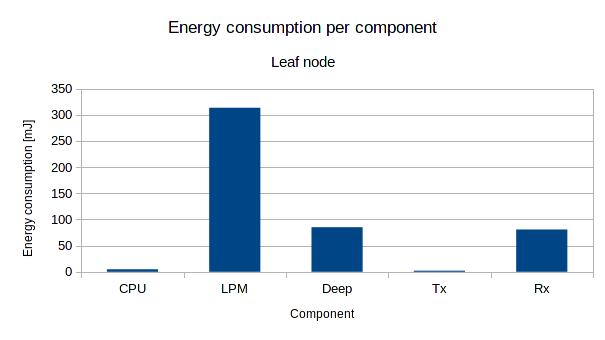
\includegraphics[width=.5\textwidth,keepaspectratio]{LeafConsumptionComponent.png}
	\caption{Zolertia leaf node average energy consumption per component.}
	\label{fig:LeafConsumptionComponent}
\end{figure}
The plotted data is available at the table \ref{tab:nodeEnergyComparison2}.
\begin{table}[H]
	\begin{center}
		\begin{tabular}{cccccc}
			\hline
			\textbf{Board} & \textbf{CPU} & \textbf{LPM} & \textbf{Deep} & \textbf{Tx} & \textbf{Rx} \\ \hline
			\textbf{Leaf}  & 4,739 mJ       & 313,51 mJ      & 85,145 mJ       & 2,135 mJ      & 80,812 mJ     \\
			\textbf{Root}  & 4,417 mJ       & 313,708 mJ     & 85,145 mJ       & 0 mJ          & 81,106 mJ     \\ \hline
		\end{tabular}
	\end{center}
	\caption{Energy consumption per component per node on average.}
	\label{tab:nodeEnergyComparison2}
\end{table}
Note that the 0 energy consumption on transmission is not due to absence of transmission on the root node, but by the fact that very few packets are transmitted hence the number is too small to be reported.
\subsection{Conclusions}
In the previous subsections, we have tested the energy consumption per component at first by only using the TSCH MAC layer, and then by enabling the full 6TiSCH stack.\\
The following table reports the total energy consumption of leaf and root note in the two scenarios.
\begin{table}[H]
	\begin{center}
		\begin{tabular}{cccl}
			\cline{1-3}
			\textbf{Board}      & \textbf{Leaf} & \textbf{Root} & \textbf{}         \\ \cline{1-3}
			\textbf{Mac only}   & 131,518 mJ      & 181,916 mJ       &                   \\
			\textbf{Full stack} & 486,341 mJ      & 484,376 mJ      &                   \\ \hline
			\textbf{}           & 269,79\%      & 166,26\%      & \textbf{Increase} \\ \hline
		\end{tabular}
	\end{center}
	\caption{Total average energy consumption of leaf and root note in the two scenarios.}
	\label{tab:scenarios1Table}
\end{table}

As it is possible to see from the table \ref{tab:scenarios1Table} the energy consumption of the two nodes following the adding of the full stack increase drastically, this is normal and predictable by the fact that adding more layers on top of the single MAC add more computational requirements to the system, so a major time spent in less energy-saving states.

\begin{thebibliography}{00}
\bibitem{inproceedings} Sabovic, Adnan \& Delgado, Carmen \& Bauwens, Jan \& De Poorter, Eli \& Famaey, Jeroen. (2019). Accurate Online Energy Consumption Estimation of IoT Devices Using Energest. 363-373. 10.1007/978-3-030-33506-9\_32. 
\end{thebibliography}

\end{document}
